\newpage
\chapter{Similar sized collisions}
\graphicspath{{./03figs/}}

Section \ref{ch07_sec01} in the appendix hababa

why are SSC non-trivial?
lot of spill-over for similar sizes
target gets changed

basic process: 

small impactor: size of impactor vs. central body field gradient small -> almost no torques

define grazing angle for each mass ratio (radii ratio)

motivation: moon formation, Lisse stuff, disks \& moons

ejecta is determined by releasing material from the surface with $v > \vesc$



% TODO: show phenomena in the angle vs. vimp plot

% TODO: plot theta_imp vs. theta_imp,core for chondritic and icy composition

% TODO: a little estimate for a toy model population in the early solar system: take 4 different sized bodies and analyze collisions into each other. make a plot with transition probabilities?

% plot accretion efficiency as a function of impact angle and compare with volumetric guess


\begin{figure}[htbp]
\begin{center}
\includegraphics[scale=0.8]{01_overview_params.pdf}
\caption{Impact geometry for a \SSC on the left side. The right plot shows a collision between a relatively small impactor compared to the target. The grazing impact angle $\theta_{graz}$ is defined as the angle for which half of the impactor simply grazes past the target \citep{Asphaug:2010p3539}. The dashed circles show the largest impact angle for which no impactor material would graze past the target $\theta_A$ and the $90^\circ$ impact angle for which the whole impactor grazes past the target. Note }
\label{ch03_fig01}
\end{center}
\end{figure}


\begin{figure}[htbp]
\begin{center}
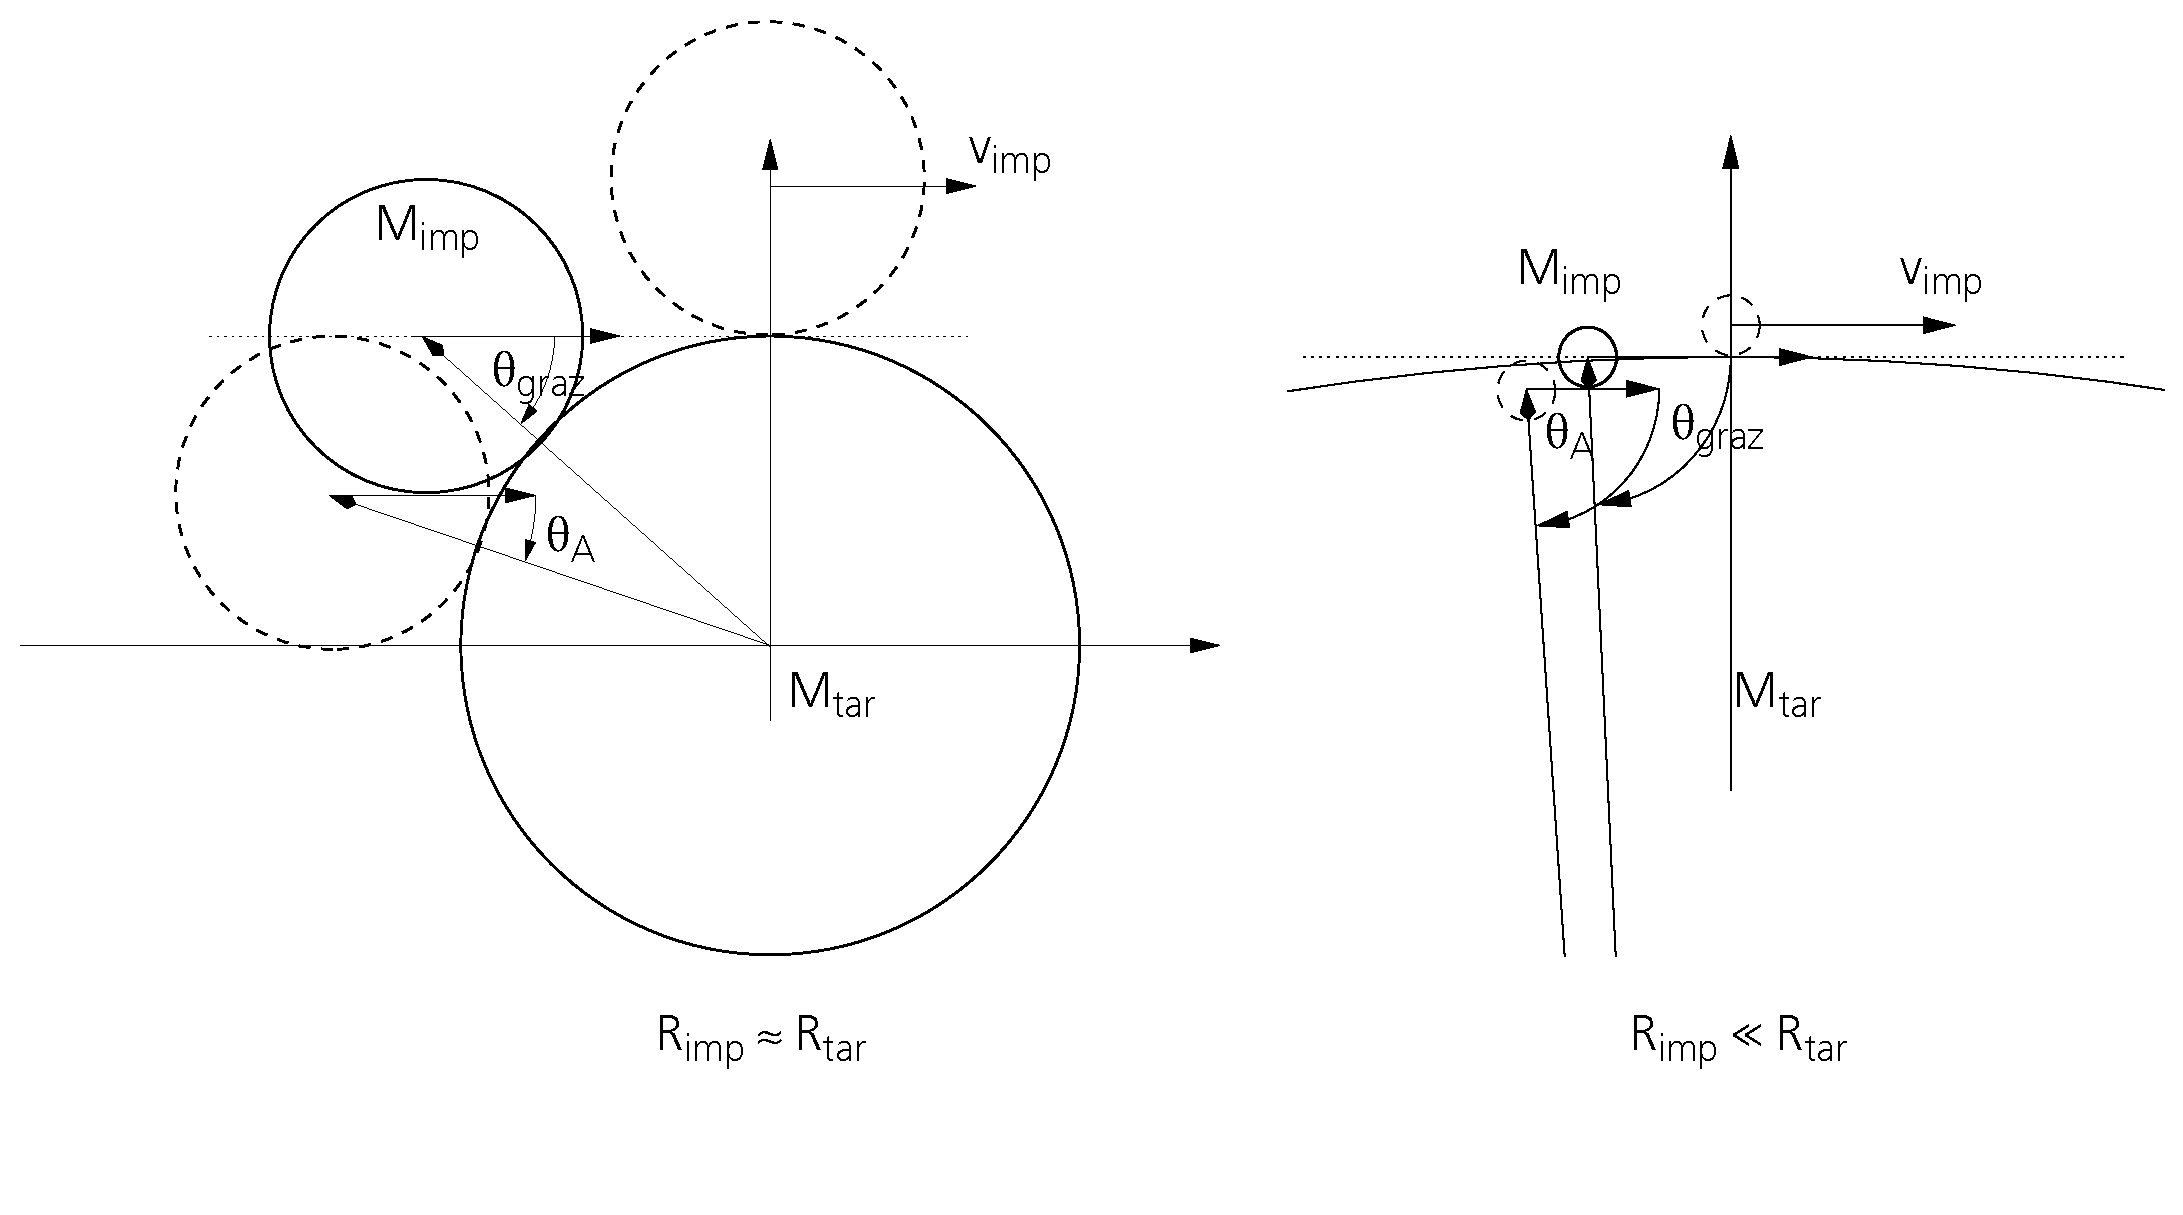
\includegraphics[scale=0.4]{03_grazing}
\caption{Impact geometry for a \SSC on the left side. The right plot shows a collision between a relatively small impactor compared to the target. The grazing impact angle $\theta_{graz}$ is defined as the angle for which half of the impactor simply grazes past the target \citep{Asphaug:2010p3539}. The dashed circles show the largest impact angle for which no impactor material would graze past the target $\theta_A$ and the $90^\circ$ impact angle for which the whole impactor grazes past the target. Note }
\label{ch03_fig01}
\end{center}
\end{figure}

\begin{equation}
\label{ch03_eq001}
\theta_{graz} = \arccos{ \frac{\Rtar}{\Rtar + \Rimp} }
\end{equation}


\begin{figure}[htbp]
\begin{center}
\includegraphics[scale=0.7]{05_Mhit}
\caption{Relative volume of the impactor ($V_{hit, imp}$, left plots) and the target ($V_{hit, tar}$, right plots) hit by the other body as a function of impact angle (top plots) and impact parameter (bottom plots) for different mass ratios $\gamma$. Compare figure \ref{ch07_fig01} for an illustration of those volumes. Note that the ratio of radii scales with the cubic root of the mass ratio: $R_{imp} / R_{tar} \sim \sqrt[3]{\gamma}$. The dotted line shows for which impact angle half of the impactor volume grazes past the target.} 
\label{ch03_fig02}
\end{center}
\end{figure}

\begin{figure}[htbp]
\begin{center}
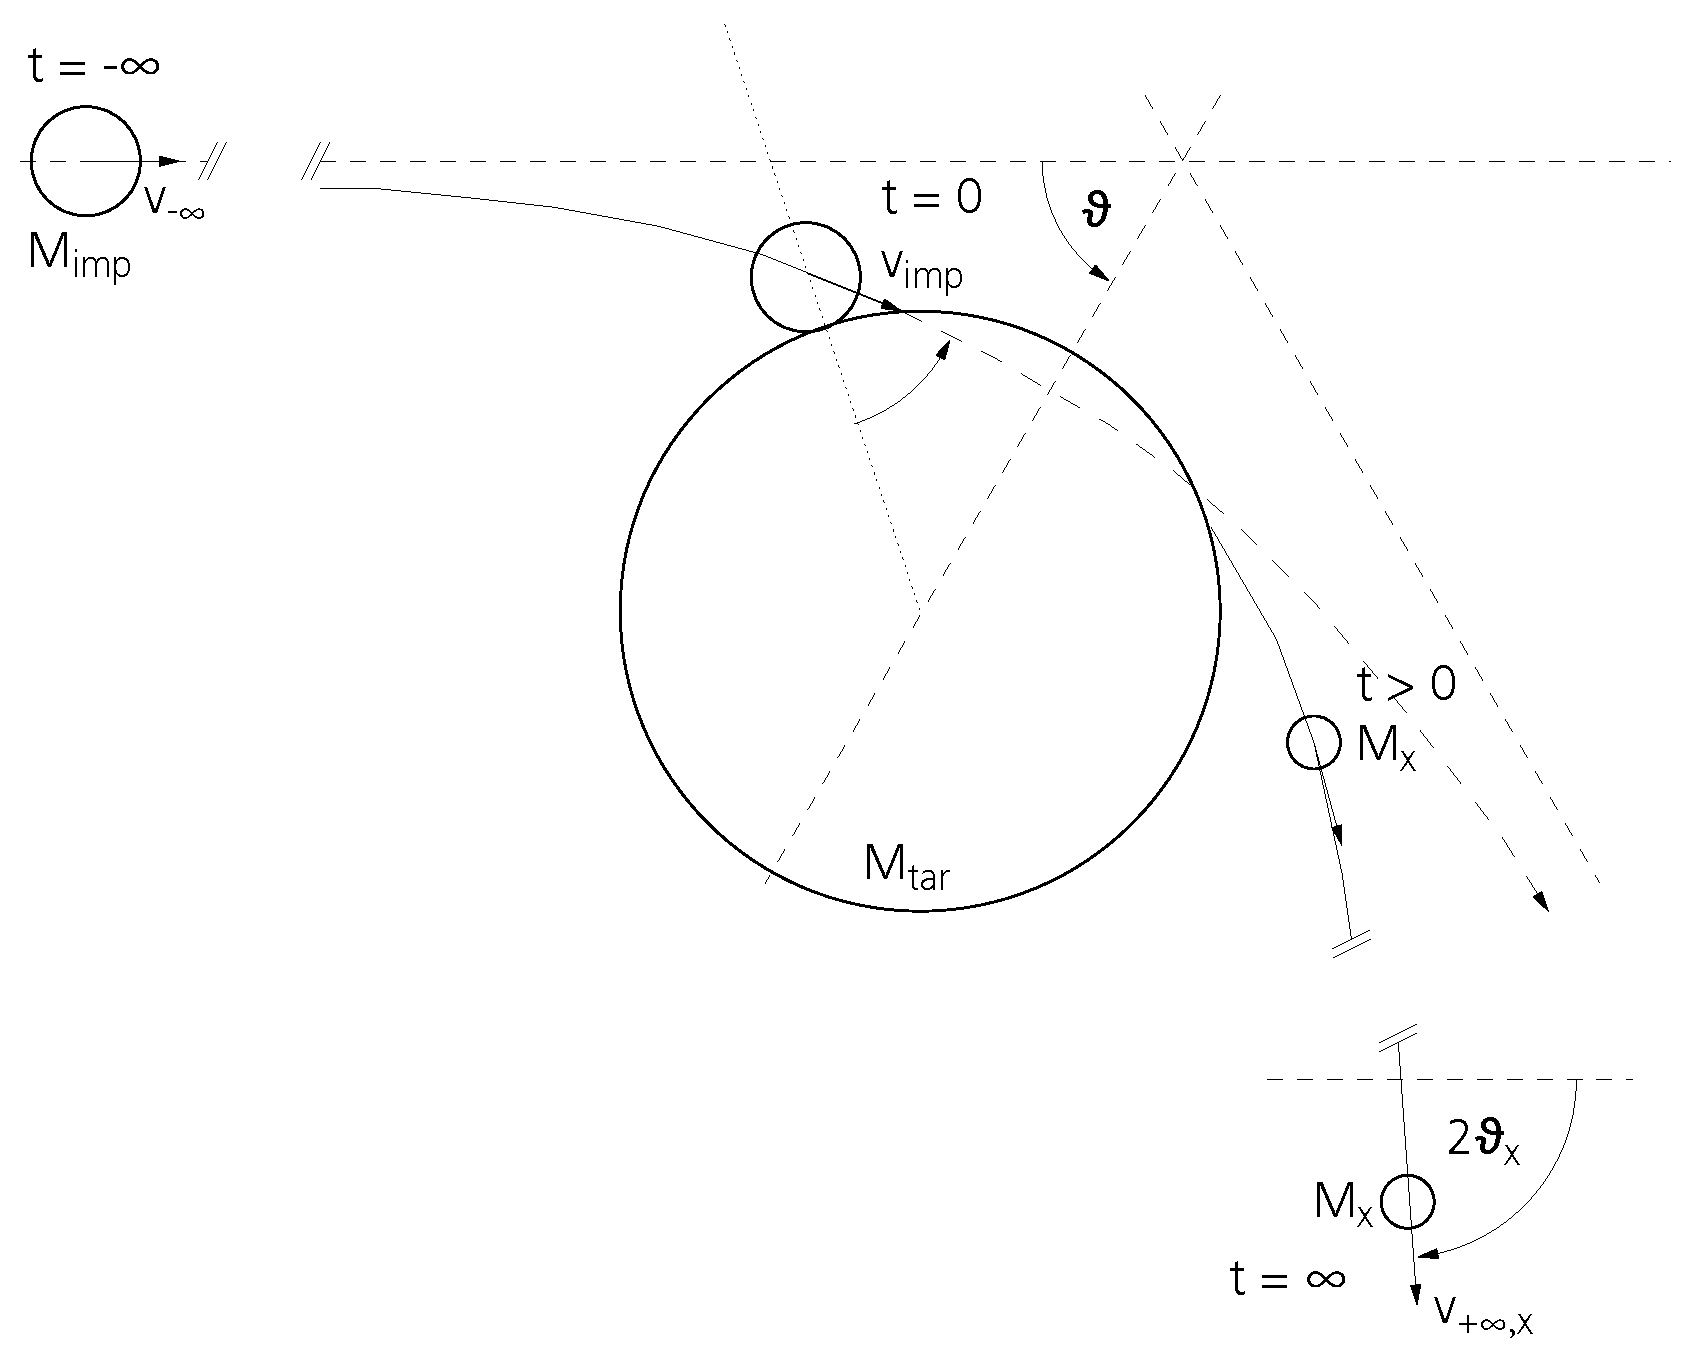
\includegraphics[scale=0.5]{04_vartheta}
\caption{Visualization of the deflection angle: The impactor approaches the target on a hyperbola (or on a parabola in case of $\vinf = 0$). Without a collision the total deflection angle of the impactor would be simply $2 \vartheta$.}
\label{ch03_fig02}
\end{center}
\end{figure}


\begin{figure}[htbp]
\begin{center}
\includegraphics[scale=0.7]{06_vimp}
\caption{An order of magnitude estimation of the random velocities for bodies undergoing collisions in a protoplanetary system with a solar mass central star. The random velocity is roughly the Kepler velocity times the orbital eccentricity. Shown are isolines of velocities for given distance from a star with a solar mass for given eccentricities. The red line shows the speed of sound of for quartz at standard conditions \cite{Melosh:2007p3502}. Note that the actual impact velocity is given by $\vimp = \sqrt{ v_{rand}^2 + \vesc^2}$ and depends on the masses of the two colliding bodies. Due to the high Kepler velocity in the inner parts of the system, even small eccentricities lead to random velocities well above the speed of sound for silicates and therefore to hypervelocity impacts even for small bodies.}
\label{ch03_fig06}
\end{center}
\end{figure}


\section{Collision physics}
compare timescales
viscous timescale $t = R^2 / \nu$
collisional timescale $t = 2 R / \vimp$
self-gravitational timescale $t = \sqrt{3\pi / G \rho}$
local gravity, free fall time
impact vs. shock velocity (super-sonic), shock waves
surface tension (Walker and Mullins 1981) vs. shearing forces, approximation of fluid bodies

\section{Review of previous work}


\section{various quantities}
accretion \& striping efficiency, compositional $\theta$ and $\xi$
angular momentum: rot. vs. pot. energy, $L_{bound}$ vs. $L_{imp}$
dynamics: deflection angle $2 \vartheta$ and $\vimp$ (momentum transfer)
energy partition, $\Delta U$
disk: mass, composition, mean a and mean e, angular momentum, compare with Kokubo moon formation scaling laws


\section{present initial conditions for the three runs}
\subsubsection{c1}
\subsubsection{i1}
when to stop

\section{\SSC categories}
show simple r3 (pure bodies)


\subsection{accretion}
\subsection{partial accretion}
\subsection{erosion \& disruption}
\subsection{hit \& run}


self-similarity when scaling impact angle vs. grazing angle and some volumetric correction?

\section{Specialities}
now show c1 \& i1
\subsection{Disks \& moon formation}

\subsection{compositional changes}
give volumetric estimate
compare icy vs. chondritic composition
introduce alternative impact angles $\theta_{core}$

\subsection{ejecta}
jetting, show decay of shock wave plot

\section{the impactor perspective}
striping efficiency


\section{interesting quantities}
\section{accretion efficiency}
\section{striping efficiency}

\cite{Chambers:2001p2105}
\citep{chandrasekhar1969ellipsoidal}
\cite{Lissauer:1993p56}
\cite{Wetherill:1993p3351}


% plots:
% impact parameter range (Mimp vs. Mtar, vimp vs. vimprel, vimp vs. angle)
% QD plot, QD*
% compositional changes
% rotational vs. potential energy and link with error in accretion efficiency

% introduce terms

% show effects: bouncing, strings of pearls, non-completion of 

%focus:
%- show parameter space, overview plot
%- chains from h&r, composition and thermodynamics of such chains
%- deflection angles for h&r, rotation (for h&r)
%- compositional changes for h&r
%- reproduce accr. efficiency in the Earth regime
%- accr. efficiencies for individual components
%- energy partition in bodies (shocks, tidal vs. self-gravity stress)
%- check Kokubo 2010 (critical velocity)
%- check Benz 1999, Angor & Asphaug 2004, Stewart & Leinhardt 2009, Marcus 2009, Marcus 2010
%- analyze ejecta, entropy and energy of ejecta
%- compare central potential of a planetary system with local gravity, compare timescales
%- analyze disk masses & composition
%- volumetric scaling (Canup 2005, Leinhardt)
%- shedding of material due to rotational ejection

\cite{Benz:1988p3336}
%- 0.1 Mearth target, 1:6 mass ratio, vimp = 2.5-8 vesc, all eroding

\cite{Benz1999Icar..142....5B}
Benz \& Asphaug 1999:
%- MLR / Mtarg ~ Q / Q*
%- parabolic fit

\cite{Canup:2000p3542}
Canup \& Agnor 2000:
%- eccentricities and masses at late stage of terrestrial planet formation
%- critical angular momentum Lcrit
%- satellite impacts are much less common due to 
	
\cite{Agnor:2004p3329}
Agnor \& Asphaug 2004: accretion efficiency during planetary collisions
%- impact probability of eps: dP = 2*sin(eps)*cos(eps)*deps (Shoemaker 1962)
%- non-disruption doesn't mean merging
%- M1: largest remnant, M2: largest escaping remnant
%- M2 / Mesc < 0.8 for 30deg -> chains
%- two 0.1Mearth mass bodies, chondritic, Tillotson
%- non-accretionary collisions are the norm

\cite{Asphaug:2006p3729}
Asphaug 2006: h\&r planetary collisions
%- 0deg: shocks dominate, 90deg gravity (tides, stresses) dominates
%- "strings of pearls"
%- for large bodies, the impactor, not the target, are destroyed
%- tidal vs. self-gravity stress inversely proportional to mass
%- relativ energy deposition 

\cite{Asphaug:2010p3539}
Asphaug 2010: SSC collisions and the diversity of planets
%- next-largest bodies (NLB)
%- hit&run common for v_rand = v_inf
%- Safronov number 1-2 in late systems
%- SSC: contact compression timescale  (2r/v_imp) on gravity timescale ( r*sqrt(G*rho) )
%- shear stress exceeds strength above 100km
%- turn-around the target reference frame: the impactor is the altered body
%- Agnor 1999: angular momentum easily above dynamical stability
%- SSC scale-invariant to the first order
%- 45deg as the median impact angle (Shoemaker 1962)
%- small r/R -> impact cratering
%- "grazing": center of impactor skims tangential to the target
%- impact cratering: angle gives all or nothing, SSC is a continuum
%- for r_core = 0.5*r -> 30deg to 90deg miss each others cores
%- h&r prevalent for NLB
%- NLBs get mantle-stripped
%- tidal disruption important for small bodies
%- icy collision might be similar to rocky ones (ice : rock ~ rock : iron)
%- iron-enriched fragments from chain-events
%- h&r happen to about half the NLB?


\cite{2009ApJ...700L.118M}
Marcus 2009:
%- confirmation of Stewart & Leinhardt 2009 for bodies > 100km
%- masses 1., 5., 10. Mearth, ratios 0.25, 0.50, 0.75
%- scaling relationship for MFe / Mlr
%- compositional changes require: a) small impact angle or b) small & fast impactor

\cite{2010ApJ...712L..73M}
Marcus et al. 2010: Minimum radii from Super-Earths: Constraints from GIs
%- super-Mercuries are not expected, as striping bodies would have to be > 10 MEarth

\cite{Stewart:2009p3265}
Stewart \& Leinhardt 2009:
%- catastrophic disruption criteria
%- Mlr / Mtarg replaced by Mlr / Mtot, Q* sclaed to reduced mass in kinetic energy

\cite{2010ApJ...714L..21K}
Kokubo \& Genda 2010:
%- about half the collisions do not accrete
%- orbit integration of 16 bodies, total mass 2.3MEarth
%- mass ratios: 1.0, 0.66, 0.50, 0.33, 0.25, 0.17, 0.11, Mtot = 0.2-2.0MEarth
%- impact velocities: 1.0-3.0 v_esc, angles: 0-75deg
%- criteria for critical impact velocity v_cr / v_esc for which accretion occurs
%- critical spin angular velocity

\cite{2011arXiv1105.4616E}
Elser et al, 2011:
%- Moon formation in planetary systems

\section{Discussion}

\bibliographystyle{plainnat}
\bibliography{bibliography}



